% \titlespacing{\chapter}{0pt}{-1\baselineskip}{\baselineskip}
\chapter{Review of Related Literature}\label{chap:RRL}
\section{On Weak and Easy Notions of Soundness in RDLTs}
As mentioned in earlier discussions, due to the dynamicity and freedom the RDLT model provides in expressing workflow in all of its dimensions, recent developments upon its formalizations have occured \cite{Malinao2017}. The concept of soundness in Workflow Nets, which implies that all of the every activity or work done by a system that can be determined in the model should exhibit proper termination and liveness, was extended to RDLT, as important of a property as it is. Although RDLT and the traditional workflow models (e.g., Workflow Nets, Business Process Management Notation, Petri Nets) differ on their syntax in presenting soundness, RDLT still adopts the conditions for soundness as discussed above. 

As in traditional workflow models, there are multiple variations to the notion of soundness, aside from the classical notion: relaxed, weak, easy, and lazy soundness. Similarly, formalizations of the definition have occured in the literature of RDLT in recent years. In \cite{MalinaoPJS2023} classical and relaxed soundness were defined along with the formalisms and design strategies. Hence, proper termination and liveness were achieved in both structural and behavioral aspects of the activities an RDLT has. The absence of such definition in the context of weak and easy soundness became the focus in Ramirez' \cite{Ramirez2024} paper. 

On the conceptual basis of the paper, \cite{Ramirez2024} initially explored the Workflow Nets, especially in the context of soundness. Weak and easy soundness, along with the other notions, in the context of workflow nets and petri nets were discussed. A weak sound RDLT requires for it to have the sink place o reachable from the source place i (option to complete), and the sink place o receives exactly one token and all other places must be empty (proper termination). In comparison to classical soundness, weak soundness is much relaxed as it does not require the involvement of every transition during execution \cite{Ramirez2024}. Similarly, it is discussed that for an RDLT to be of easy sound, its sink place o should be reachable from source place i (option to complete). %% TODO: find the requirements for the conditions for it to be weak and easy sound %%

This definition was then extended in\cite{Ramirez2024} in the formalizations of weak and easy soundness in the context of RDLT, hence the following definitions.

\begin{defn}[\textbf{Weak Soundness of RDLTs}] 
    \label{WeakRDLTDef}
    An RDLT $ R $ is of weak soundness if and only if the following requirement is satisfied by each activity profile $ S = \{S(1), S(2), \ldots S(k)\}, 1 \leq k \leq diam(R), diam(R) $ is the diameter of $ R $, of a set of source vertices $ I $ $ \subset $ $ V $ and a final output vertex $ f $ $ \in $ $ V, $ where $ \forall $ $ x $ $ \in $ $ I $ and $ y $ $ \in $ $ V $, $ (x,y) $ $ \in $ $ S(1), $ and $ (u,f) $ $ \in $ $ S(k) $, $ u $ $ \in $ $ V $:
    \begin{enumerate}
        \item \textbf{Proper termination.} For every activity profile $ S = \{S(1), S(2), \ldots S(k)\}, 1 \leq k \leq diam(R) $, of a set of source vertices $ I $ $ \subset $ $ V $ and a final output vertex $ f $ $ \in $ $ V $.
        \begin{itemize}
            \item All arcs in the final reachability configuration $ S(k) $ must be incident to sink $ f $, i.e. for every $ (x,y) $ $ \in $ $ S(k), $ $ y = f $
            \item If $ k $ $ \leq $ $ 2 $: every arc incident to a vertex $ y $ in a reachability configuration $ S(i) $ has a corresponding arc incident from vertex $ y $ in a succeeding reachability configuration $ S(j) $, i.e.\ for every $ (x,y) $ $ \in $ $ S(i) $, there exists another arc $ (y,z) $ $ \in $ $ S(j) $, for all $ 1 \leq i < k $, and for some $ j $ in the range $ i + 1 \leq j \leq k $.
        \end{itemize}
    \end{enumerate}
\end{defn}
Based on this definition, an RDLT is of weak soundness if it properly terminates, where every reached vertex in each activity profile of the RDLT leads to the sink. In the context of WF-Nets, this notion of soundness in RDLT is similar in a sense that it does not require the workflow to be live. A weak sound RDLT allows for arcs to not be traversed at all. \\
In figure\ref{RDLTWeak}, a weak sound RDLT is shown. All the arcs leading to $x_5$ from $x_4$ can be traversed, except with the path starting from the arc $(x_1, x_2)$, since it cannot be traversed.
\begin{figure}[H]
    \centering
    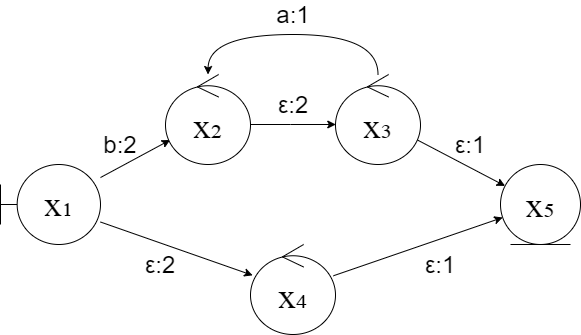
\includegraphics[width=12cm]{figures/RDLT Weak.png}
    \caption{An RDLT of Weak Soundness (Image Source:\cite{Ramirez2024})}\label{RDLTWeak}
\end{figure}

The structural profile as defined by\cite{Ramirez2024} of a weak sound RDLT is summarized by the following theorem:
\begin{thm}\textbf{Structural Verification of the Weak Soundness of an RDLT $ R $}\label{SVWeak}
\cite{Ramirez2024}
    An RDLT $ R $ is weak-sound if and only if both the level-1 and level-2 expanded vertex simplifications of R, $ R_1 $ and $ R_2 $ respectively, are deadlock-tolerant.
\end{thm}

The algorithm\ref{WeakAlg} for the verification of weak soundness in RDLT is at the appendices.

On the verification of weak soundness in RDLT, it its stated at theorem\ref{SVWeak} that both expanded vertex simplifications of $R$, should be deadlock tolerant. To understand deadlock tolerance, the following definitons are stated. The following are sourced from \cite{Ramirez2024} unless otherwse stated.

\begin{defn}\textbf{Weakened JOIN-safe RDLT $ R $}\cite{Ramirez2024}\label{WJRDLT}
    An RDLT $ R $ is weakened JOIN-safe if every split-join pair in $ R $ has weakened JOIN-safe $ L $-values.
\end{defn}

\begin{defn}\textbf{Deadlock Point}
    \cite{Ramirez2024}
    \label{DLP}
    A deadlock point is each vertex $ x $ $ \in $ $ dV $ in an RDLT $ R $ where $ dV $ is a set of vertices in $ R $ and $ dV $ $ \subset $ $ V $, such that $ x $ $ \in $ $ dV $ is unreachable at some time step of the activity extraction algorithm.
\end{defn}

\begin{defn}\textbf{Escape Contraction Path}
    \cite{Ramirez2024}
    \label{ECPath}
    An escape contraction path is a path $ P = x_1, x_2 \ldots x_n $ in an RDLT $ R $ such that the following holds:
    \begin{enumerate}
        \item $ x_1 $ is a parent of a deadlock point in $ R $, i.e. $ x_1 $ $ = $ $ p $ where $ (p,q) $ $ \in $ $ E $ and $ q $ $ \in $ $ dV $, and
        \item $ P $ is a contraction path from $ x_1 $ to $ x_n $ in $ R $ where $ x_n $ is the sink vertex of $ R $.
    \end{enumerate}
\end{defn}

\begin{defn}\textbf{Deadlock-Resolving RDLT $ R $}
    \label{DLResolving}
    \cite{Ramirez2024}
    An RDLT $ R $ is deadlock-resolving if for every deadlock point $ x \in V $, there exists at least one escape contraction path from a parent of $ x $ to the sink in R.
\end{defn}

\begin{lem}
    \cite{Ramirez2024}
    An expanded vertex simplification $ R_i $, where $ i $ $ = $ $ 1, 2 $, is deadlock-tolerant if and only if every activity thereof properly terminates.
\end{lem}

\begin{defn}\textbf{Deadlock-Tolerant RDLT $ R $}
    \cite{Ramirez2024}
    An RDLT $ R $ is deadlock-tolerant if every NCA is loop-safe, every CA is safe, $ R $ is weakened JOIN-safe and deadlock-resolving.
\end{defn}

% ---------------------------
% Easy Soundness Notion of RDLTs
\subsection*{Easy Soundness Notion of RDLTs}

\begin{defn}\textbf{Self-Controlling Arc} \\
    \cite{Ramirez2024}
    \label{SelfCA}
    A self-controlling arc is a profile of an RDLT $ R $ where a MIX-JOIN or AND-JOIN at vertex $ x $ can never be resolved. 
\end{defn}

Figure \ref{SelfControllingArc}, shown below, is an example of a self-controlling arc as defined in Definition \ref{SelfCA}. In this case, vertex $ b $ is the vertex that can never resolved due to one of the components of the AND-JOIN that violates the unconstrainedness criterion of the activity extraction algorithm.

\begin{figure}[H]
    \centering
    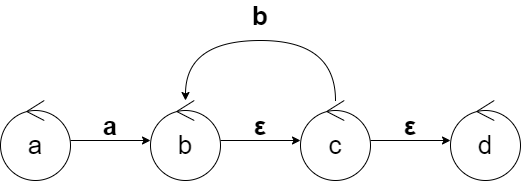
\includegraphics[width=12cm]{figures/Self-Controlling Loop.png}
    \caption{An RDLT a Self-Controllin Arc Image Source: \cite{Ramirez2024}}
    \label{SelfControllingArc}
\end{figure}

\begin{defn}\textbf{Easy Soundness of RDLTs}
    \label{EasyRDLTDef}
    \cite{Ramirez2024}
    An RDLT $ R $ is of easy soundness if and only if the following requirement is satisfied by an existing activity profile $ S = \{S(1), S(2), ..., S(k)\}, 1 \leq k \leq diam(R), diam(R) $ is the diameter of $ R $, of a set of source vertices $ I $ $ \subset $ $ V $ and a final output vertex $ f $ $ \in $ $ V, $ where $ \forall $ $ x $ $ \in $ $ I $ and $ y $ $ \in $ $ V $, $ (x,y) $ $ \in $ $ S(1), $ and $ (u,f) $ $ \in $ $ S(k) $, $ u $ $ \in $ $ V $:
    \begin{enumerate}
        \item \textbf{Option to complete.} There exists an activity profile $ S = \{S(1), S(2), ..., S(k)\}, 1 \leq k \leq diam(R) $, of a set of source vertices $ I $ $ \subset $ $ V $ and a final output vertex $ f $ $ \in $ $ V $ where there exists a path $ P $ composed of $ P = x_1, x_2 \cdots x_n $ with $ i = 1, 2 \cdots n - 2 $ where $ (x_i, x_{i+1}) $ $ \in $ $ S(i), (x_{i+1}, x_{i+2}) $ $ \in $ $ S(j), i < j, x_i = s $ and $ x_n = f $.
    \end{enumerate}
\end{defn}

\begin{figure}[H]
    \cite{Ramirez2024}
    \centering
    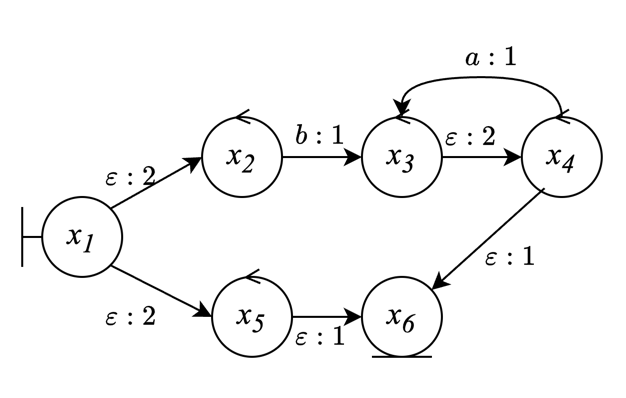
\includegraphics[width=12cm]{figures/easySoundRDLT.png}
    \caption{An RDLT of Easy Soundness}
    \label{RDLTEasy}

\end{figure}

Based on this definition, the RDLT in Figure \ref{RDLTEasy} is of easy sound.

Shown below is Theorem \ref{SVEasy} that describes the structural requirements required to determine the easy soundness of an RDLT.

\begin{thm}\textbf{Structural Verification of the Easy Soundness of an RDLT $ R $}
    \cite{Ramirez2024}
    \label{SVEasy}
    An RDLT $ R $ is easy-sound if and only if the following elements exist: 
    \begin{itemize}
        \item A contraction path $ P_1 $ in the level-1 vertex simplification $ R_1 $ of $ R $ from the initial vertex $ x_i $ to the final vertex $ x_f $, wherein $ P_1 $ $ = $ $ x_1, \ldots, x_f $
        \item A contraction path $ P_2 $ in the level-2 vertex simplification $ R_2 $ of $ R $ from the initial vertex $ z $ to the final vertex $ p $ of the RBS, wherein $ P_2 $ $ = $ $ z, \ldots, p $
        \item An in-bridge $ (x,y) $ formed by a component in $ P_1 $ such that there exists a component $ (y,z) $ in $ P_2 $
        \item An out-bridge $ (q,p) $ formed by a component in $ P_2 $ such that there exists a component $ (p,r) $ in $ P_1 $
    \end{itemize}
\end{thm}

%% TODO: Include a illustration of the application of the algorithm on the said RDLT %%

% The process shows that the expanded vertex simplified graph \mathcal{R_1}
% %TODO: edit all the equations %
% produced at step 7, only one deadlock-point was identified: x_2. The stored deadlock points (in this case, only one vertex x_1) will be checked of a non-critical loop-safe escape contraction path, as defined in Definition \ref{criticalArc} \ref{loopSafe} \ref{escapeContractionPath} 
% %TODO: Include all these definitions %
% from that vertex.  Every split-join pair with respect to x_1 is also checked if they have a weakened JOIN-safe L-values as defined in Definition \ref{weakenedJoinSafeLValues} 
% % TODO: Include reference to definitions%.  
% And since this deadlock point has a non-critical loop-safe contraction path existing, and the split-join pair (or just the arc) containing the deadlock point has weakened JOIN-safe L-values, the vertex simplified graph is deadlock tolerant. Hence, the algorithm return the boolean true.  //
% The time complexity of WRSVA is domininated by the loop-safeness checks, deadlock point identification, and escape contraction path verificaiton. Vertex simplification, including expanded vertex simplification, contributes to the time complexit proportional to the number of vertices and arcs in the original RDLT. The iteration through all vertices to identify potential deadlock points has a linear time complexity with respect to the number of vertices, O(|V|). 
% TODO: add equation for this time complexity %
% For each loop and identified deadlock point, the algorithm checks for loop-safeness and verifies escape contraction paths. This involves analyzing arcs and traversla limits, and is intensive in computation due to nested iteratinos. Hence, the overall time complexit is O(c⋅∣E∣4) %% TODO: proper equation %%
%  where c is a constant accounting for the complexit of loop-safeness checks, and E is the number of arcs in the RDLT.  In terms of space complexity, WRSVA is approximately O(c∣E∣) which is linear with respect to the size of the RDLT. Of course, with actual data structures to store these graphs and identified paths and vertices, the space complexity is subject to change. 

% The conditions for an easy sound RDLT are explained in Theorem \ref{easyStructureTheorem}. The algorithm EVRSA is also detailed in Algorithm \ref{EVRSA}. To illustrate this activity, we take a look at Figure \ref{parallelEasyRDLT}, and it is proven that the RDLT is indeed of easy soundness. For every vertex simplification of the RDLT R, the graph contraction strategy, as defined in Definition \ref{graphContraction}
% %  TODO: add graph contraction reference %
% is applied. The algorithm proceeds with checking if the simplified vertex R_1 has a contraction path from the source x-1 to the sink x_n, and if it does (for every level of vertex simplification) then the algorithm will return true, otherwise false. This verifies the easy soundness of the RDLT. 

% The time and space complexity of ERSVA is explained in theorem \ref{theoremERSVA}. It is detailed that the algorithm has a time complexity of O(|V^2|), and a space complexity of O(|V^2|) as well, with the procedure mainly focusing on vertec simplification and graph contraction.

\section{On Verification Strategies of Soundness Properties of RDLT}
\subsection*{Matrix Representation and Automation of Verification of Soundness of Robustness Diagram with Loop and Time Controls}
In their paper titled \emph{"Matrix Representation and Automation of Verification of Soundness of Robustness Diagram with Loop and Time Controls"} Karen and Roben \cite{KarenRoben2018} proposed a matrix representation for the verification of soundness of RDLT. They used matrix representations for the state of the $R$ during activity extraction. The verification of soundness, then, is done by analyzing the \emph{final state vector} resulting from ${\mathcal{A}}$ they incorporated from \cite{Malinao2017}. Their methodology is shown to be effective in verifying \emph{relaxed soundness} property of an RDLT. 
The following are the basic concepts and definitions necessary to understand the verification of soundness property of RLDT through matrix verification. The formal definition of these vectors and matrix operations are from \cite{KarenRoben2018} unless stated otherwise.

\begin{defn}\label{def:counter_vector}
    \textit{\textbf{Counter Vector} \cite{KarenRoben2018}\\
    Let $R = (V, E, \Sigma, C, L, M)$ be an RDLT and $Q = (e_{1}, e_{2}, \ldots, e_{q})$ be the finite sequence of arcs in $R$ where $q = |E|$ and $e_{i} \in E$ is the i\textsuperscript{th} arc of the sequence. The counter vector at time step $t$ is defined as
    \begin{displaymath}
    \alpha(t) = ({a_{1}}^{(t)}, {a_{2}}^{(t)}, \ldots, {a_{q}}^{(t)})
    \end{displaymath}
    such that ${a_{i}}^{(t)} \in \mathbb{N}$ represents the total number of times arc $e_{i}$ has been explored from time step 0 to time step $t$.}
    \end{defn}
    
    \begin{defn}\label{def:constraint_vector}
    \textit{\textbf{Constraint Vector} \cite{KarenRoben2018}\\
    Let $R = (V, E, \Sigma, C, L, M)$ be an RDLT and $Q = (e_{1}, e_{2}, \ldots, e_{q})$ be the finite sequence of arcs in $R$ where $q = |E|$ and $e_{i} \in E$ is the i\textsuperscript{th} arc of the sequence. The constraint vector at time step $t$ is defined as
    \begin{displaymath}
    \beta(t) = ({b_{1}}^{(t)}, {b_{2}}^{(t)}, \ldots, {b_{q}}^{(t)})
    \end{displaymath}
    such that 
    \begin{displaymath}
    {b_{i}}^{(t)} = 
    \left\{
    \begin{array}{rl}
       C(e_{i})_{y}, &\text{if (arc $e_{i}$ is currently checked but cannot yet}\\
       &\text{be traversed at time step $t$) or (arc $e_{i} = (x,y)$}\\
       &\text{with $C(e_{i}) = \epsilon$ is not checked but there exists}\\
       &\text{arc $e_{j} = (v,y)$ that is currently checked)}\\
       &\text{where $C(e_{i})$ is the attribute C of arc $e_{i}$;}\\
       -C(e_{i})_{y}, &\text{if arc $e_{i} = (x,y)$ with $C(e_{i}) \in \Sigma$ is not checked}\\
       &\text{but there exists arc $e_{j} = (v,y)$ that is currently}\\ 
       &\text{checked where $C(e_{i})$ is the attribute C of arc $e_{i}$;}\\ 
       0_{y}, &\text{otherwise.}
    \end{array}
    \right.
    \end{displaymath}}
    \end{defn}
    
    \begin{defn}\label{def:state_vector}A
    \textit{\textbf{State Vector} \cite{KarenRoben2018}\\
    %Let $R = (V, E, \Sigma, C, L, M)$ be an RDLT, $Q = (e_{1}, e_{2}, \ldots, e_{q})$ be the finite sequence of arcs in $R$ where $q = |E|$ and $e_{i} \in E$ is the i\textsuperscript{th} arc of the sequence, $\alpha(t)$ be the counter vector at time step $t \in \mathbb{N}$, and $\beta(t)$ be the constraint vector at time step $t \in \mathbb{N}$. 
    Let $\alpha(t)$ be the counter vector at time step $t$ and $\beta(t)$ be the constraint vector at time step $t$. The state vector at time step $t$ is defined as 
    \begin{displaymath}
    \rho(t) = \small[\alpha(t),\beta(t)\small].
    \end{displaymath}}
    \end{defn}
    
    Aside from the vectors defined above, \cite{KarenRoben2018} also conceptualized the use of matrix to keep track of the steps done during activity extraction, that is the arcs explored at every time step $t$. These are the components for \emph{activity extraction} using matrix representation:

%   -----
%  COMPONENTS FOR ACTIVITY EXTRACTION
\begin{defn}\label{def:explored_vector}
    \textit{\textbf{Explored Arcs Vector}\\
    Let $R = (V, E, \Sigma, C, L, M)$ be an RDLT and $Q = (e_{1}, e_{2}, \ldots, e_{q})$ be the finite sequence of arcs in $R$ where $q = |E|$ and $e_{i} \in E$ is the i\textsuperscript{th} arc of the sequence. The explored arcs vector at time step $t$ is defined as
    \begin{displaymath}
    \gamma(t) = ({g_{1}}^{(t)}, {g_{2}}^{(t)}, \ldots, {g_{q}}^{(t)})
    \end{displaymath}
    such that 
    \begin{displaymath}
    {g_{i}}^{(t)} = 
    \left\{
    \begin{array}{rl}
       1, &\text{if arc $e_{i} = (x,y)$ is chosen to be explored at time}\\
       &\text{step $t$ where vertex $x$ was already reached before}\\
       &\text{time step $t$;}\\
       0, &\text{otherwise.}
    \end{array}
    \right.
    \end{displaymath}}
    \end{defn}
    
    % When $(x,y) \in E$ is explored at $t$, the constraint of every incoming arc $(v,y) \in E$ of vertex $y \in V$ determines whether $(x,y)$ will only be checked at $t$ or will be traversed at $t$. In this paper, the incoming arcs vector is defined to represent these incoming arcs. Also, the C-attribute vector is defined to represent the constraint of every arc in $R$. It must be recalled that $\epsilon$ represents a constraint-free process flow. Thus, $(v,y)$ does not prevent the traversal of $(x,y)$ when $C((v,y)) = \epsilon$.
    
    \begin{defn}\label{def:incoming_arcs_vector}
    \textit{\textbf{Incoming Arcs Vector}\\
    Let $R = (V, E, \Sigma, C, L, M)$ be an RDLT, $Q = (e_{1}, e_{2}, \ldots, e_{q})$ be the finite sequence of arcs in $R$ where $q = |E|$ and $e_{i} \in E$ is the i\textsuperscript{th} arc of the sequence, and $\gamma(t) = ({g_{1}}^{(t)}, {g_{2}}^{(t)}, \ldots, {g_{q}}^{(t)})$ be the explored arcs vector at time step $t$. The incoming arcs vector at time step $t$ is defined as
    \begin{displaymath}
    \phi(t) = ({p_{1}}^{(t)}, {p_{2}}^{(t)}, \ldots, {p_{q}}^{(t)})
    \end{displaymath}
    such that 
    \begin{displaymath}
    {p_{i}}^{(t)} = 
    \left\{
    \begin{array}{rl}
       1, &\text{if $({g_{i}}^{(t)} = 1)$ or $({g_{i}}^{(t)} = 0$ and $C(e_{i}) = \epsilon_{y}$ and}\\
       &\text{$\exists{g_{j}}^{(t)} = 1)$ where $e_{i} = (x,y), e_{j} = (v,y),$ and $C(e_{i})$}\\
       &\text{is the attribute C of arc $e_{i}$;}\\
       -1, &\text{if ${g_{i}}^{(t)} = 0$ and $C(e_{i}) \in \Sigma$ and $\exists{g_{j}}^{(t)} = 1$ where}\\
       &\text{$e_{i} = (x,y), e_{j} = (v,y),$ and $C(e_{i})$ is the attribute C}\\
       &\text{of arc $e_{i}$;}\\
       0, &\text{otherwise.}
    \end{array}
    \right.
    \end{displaymath}}
    \end{defn}
    
    \begin{defn}\label{def:C-attribute_vector}
    \textit{\textbf{C-Attribute Vector}\\
    Let $R = (V, E, \Sigma, C, L, M)$ be an RDLT and $Q = (e_{1}, e_{2}, \ldots, e_{q})$ be the finite sequence of arcs in $R$ where $q = |E|$ and $e_{i} \in E$ is the i\textsuperscript{th} arc of the sequence. The C-attribute vector of $R$ is defined as
    \begin{displaymath}
    \vec{C} = (c_{1}, c_{2}, \ldots, c_{q})
    \end{displaymath}
    such that $c_{i} = C(e_{i})_{y}$ where $C(e_{i})$ is the attribute C of $e_{i} = (x,y)$.}
    \end{defn}
%   -----

    To describe $R$ fully at each time step, the constraints of the arcs are also monitored, through an \textbf{unrefreshed constraint vector}, which at time step $t$ shows which among the constraints of the arcs in $R$ are satisfied. The formal definition is described below:

    \begin{defn} \textbf{Unrefreshed Constraint Vector} \cite{KarenRoben2018} \\
        Let $\beta(t-1)$ be the constraint vector at time step $t-1$, $\phi(t)$ be the incoming arcs vector at time step $t$, and $\vec{C}$ be the $C$-attribute vector of $R$. The unrefreshed constraint vector at time step $t$ is defined as
        \[
        \omega(t) = \beta(t-1) \lor \big(\phi(t) \odot \vec{C}\big).
        \]       
    \end{defn}
    
    Similarly, The \textbf{refresh vector} is introduced to ensure that the constraints for reaching a vertex $y$ are reset or refreshed once the vertex is reached. 
    \begin{defn} \textbf{Refresh Vector} \cite{KarenRoben2018} \\
        Let $\omega(t) = \big(w_1^{(t)}, w_2^{(t)}, \dots, w_q^{(t)}\big)$ be the unrefreshed constraint vector at time step $t$. The refresh function of `$\omega(t)$ is defined as
        \[
        \text{refresh}(\omega(t)) = Z
        \]
        where $Z = \big(z_1, z_2, \dots, z_q\big)$ such that
        \[
        z_i =
        \begin{cases}
        0_y, & \text{if } e_i = (x, y) \text{ is traversed at time step } t; \\
        w_i, & \text{if } e_i \text{ cannot yet be traversed at time step } t.
        \end{cases}'
        \]
    \end{defn}
    
    These vectors are supported by the matrix operations estabilished by \cite{KarenRoben2018}, namely: \textbf{Literal Sign Function}, \textbf{Literal OR}, and \textbf{Literal Element-Wise Multiplication}.

    Ultimately, these matrix representations and operations yield a final state vector, upon which properties of soundness can be analyzed, hence be verified.

    \subsection*{Automated Verification of Classical Soundness in Robustness Diagrams with Loop and Time Controls via L-safeness}
    On their paper titled \textit{"Automated Verification of Classical Soundness in Robustness Diagrams with Loop and Time Controls via $L$-safeness"}, Asoy \cite{Asoy2024} proposed a system for the automated verification of Classical Soundness of RDLT \cite{MalinaoPJS2023}. In this paper, they utilized the idea, and other defined vectors, of a Matrix-based verification of the propery of soundness, from the paper of Karen and Roben \cite{KarenRoben2018}. \\
    
    A summary of the methodology is as follows. An input RDLT is processed by the system to generate expanded vertex simplifications, either level-1 or level-2, depending on the existence of an RBS. Then, through $L$-safeness verification, the system performs generation of matrices and related matrix operations to verify the conditions of the $L$-safeness of the simplified RLDT's, of which's conclusion, if either classically sound or not, be generalized to the original input RLDT. \\

    Asoy \cite{Asoy2024} was able to propose several algorithms that helped for the verificaion of the conditions of an $L$-safe RDLT. The following includes an algorithm for the generation of level-1 (or level-2) expanded vertex simplification, producing also \textit{abstract arcs}, which is an arc that connects an $R_2$ vertex with an in-bridge or out-bridge, aggregating the $l$-attributes of tha arc across multiple arcs it is involved; an algorithm for determining the \textit{loop-safeness} of an $NCA$; conversion of the expanded vertex simplfied graph to its corresponding matrix form, which is composed of the vectors $C$-attribute, $L$-attribute, $eRU$ for all of the arcs; for the verification of \textit{safeness of Critical Arcs}; and, finally, for the verification of $L$-safeness and Classical soundness of the simplified RDLT, hence the original input RDLT. \\

    The vectors utilized in this system are: the first aforementioned vectors storing the $C$-attribute, $L$-attribute, and $eRU$ of each arcs; \textit{Cycle Vector}, which indicates whether an arc is a part of a cycle (1 if the arc is part of a cycle but not a critical arc, -1 if is a part of a cycle and is a critical arc, and 0 otherwise); the \textit{Out Cycle Vector}, which indicates the existince of escape non-critical arc for a critical arc (C if a critical arc has an escape NCA, -C if it has an escape arc, but not NCA, and 0 otherwise); a vector for $loop-safeness$, which shows if an NCA can be reused as many times as it is required from all the cycles it is associated with, provied its value on the cycle vector is 1, or if its part of a cycle (1 if $L$-attribute is greater than $eRU$, -1 if $L$-attribute is less than $eRU$, 0 otherwise); vector for safeness of a Critical arc; and several others for the verification of the JOIN-safeness of RDLT. \\

    Asoy \cite{Asoy} was able to utilize all of these vectors through a matrix and apply related operations for the verification of properties of an $L$-safe RDLT. On top of that, they were also able to generate the components of the RDLT upon which violations were detected during the execution of the aforementioned operations. \\

    In summary, the utitlization of matrices in the verification of properties of an RDLT is an effective method, along with the consideration of the time and space complexity of the algorithms. In relation to this current research, the idea of using matrix-based verification of weak and easy soundness, just like in the verification of classical soundness in RDLT, is plausible and meritous idea, to which the study will be modifying to suit the structural characteristics of a weak and easy sound RDLT. \\